\documentclass{ctuthesis}
\usepackage{graphicx}
\usepackage{lipsum}                     
\usepackage{xargs}                     
\usepackage[pdftex,dvipsnames,usenames,nonamebreak]{xcolor}
\usepackage[colorinlistoftodos,prependcaption,textsize=tiny]{todonotes}
\newcommandx{\unsure}[2][1=]{\todo[linecolor=red,backgroundcolor=red!25,bordercolor=red,#1]{#2}}
\newcommandx{\change}[2][1=]{\todo[linecolor=blue,backgroundcolor=blue!25,bordercolor=blue,#1]{#2}}
\newcommandx{\info}[2][1=]{\todo[linecolor=OliveGreen,backgroundcolor=OliveGreen!25,bordercolor=OliveGreen,#1]{#2}}
\newcommandx{\improvement}[2][1=]{\todo[linecolor=Plum,backgroundcolor=Plum!25,bordercolor=Plum,#1]{#2}}
\newcommandx{\thiswillnotshow}[2][1=]{\todo[disable,#1]{#2}}

\def\justifying{%
	\rightskip=0pt
	\spaceskip=0pt
	\xspaceskip=0pt
	\relax
}
\usepackage{subfig}
\usepackage{multicol}
\usepackage{tcolorbox}
\usepackage{tabularx}
\usepackage{array}
\usepackage{tikz}
\def\checkmark{\tikz\fill[scale=0.4](0,.35) -- (.25,0) -- (1,.7) -- (.25,.15) -- cycle;}
\usepackage{colortbl}
\tcbuselibrary{skins}
%\newcolumntype{Y}{>{\raggedleft\arraybackslash}X}
\tcbset{tab2/.style={enhanced,fonttitle=\bfseries,fontupper=\normalsize\sffamily,
		colback=yellow!10!white,colframe=red!50!black,colbacktitle=Salmon!40!white,
		coltitle=black,center title}}

%\usepackage{csquotes}
%\renewcommand*{\labelalphaothers}{}
%
%\DeclareLabelalphaTemplate{
%	\labelelement{
%		\field[final]{shorthand}
%		\field{label}
%		\field{labelname}
%	}
%	\labelelement{
%		\literal{\string\space}
%	}
%	\labelelement{
%		\field{year}
%	}
%}

%\addbibresource{refs.bib}



\ctusetup{
	xdoctype = B,
	xfaculty = FCEyN,
	mainlanguage = czech,
	titlelanguage = czech,
	title-english = {},
	title-czech = {Construcción e implementación de un sistema integral de 
		caracterización de filtros ópticos de interferencia de banda utilizados en 
		cámaras 
		hiperespectrales.},
	department-czech = {Departamento de Física},
	author = {Juan Reto Reynal},
	supervisor = {Prof. Dr. Hernán Grecco},
	supervisor-address = {Laboratorio de Electrónica Cuántica, DF, FCEyN, UBA.},
	month = 4,
	year = 2020,
}


\ctuprocess





\def\ctucaptionsenglish{
	\def\appendicesname{Appendices}
	\def\thanksname{}
	\def\abstractname{Abstract}
	\def\declarationname{}
	\def\listfigurename{Figures}
	\def\listtablename{Tables}
	\def\supervisorname{Supervisor}
	\def\supervisorspecialistname{Supervisor--specialist}
	\def\fieldofstudyname{Field\ of\ study}
	\def\subfieldofstudyname{Subfield}
	\def\specificationname{Project\ Specification}
	\def\keywordsname{Keywords}
	\def\titletranslationname{Title\ translation}
}

\def\ctucaptionsczech{
	\def\appendicesname{Apéndice}
	\def\thanksname{}
	\def\contentsname{Índice}
	\def\abstractname{Resumen}
	\def\declarationname{}
	\def\listfigurename{Índice de Figuras}
	\def\listtablename{Índice de Tablas}
	\def\supervisorname{Director}
	\def\supervisorspecialistname{\v Skolitel--specialista}
	\def\fieldofstudyname{Obor}
	\def\subfieldofstudyname{Zam\v e\v ren\'i}
	\def\specificationname{Zad\'an\'i\ pr\'ace}
	\def\keywordsname{Palabras clave}
	\def\titletranslationname{P\v reklad\ n\'azvu}
}



\begin{thanks}
	
	\raggedright
	\textsc{TEMA:} Construcción e implementación de un sistema integral de caracterización de filtros ópticos utilizados en cámaras hiperespectrales.
	
	\bigskip
	
	\textsc{ALUMNO:} Juan Reto Reynal
	
	\bigskip
	
	\textsc{L.U. N$^{\circ}$:} 777/12
	
	\bigskip
	
	\textsc{LUGAR DE TRABAJO:} LEC, Departamento de Física, FCEyN, UBA.
	
	
	\bigskip
	
	\textsc{DIRECTOR DEL TRABAJO:} Dr. Hernán E. Grecco
	
	\bigskip
	
	\textsc{FECHA DE INICIACIÓN:} Abril de 2019
	
	\bigskip
	
	\textsc{FECHA DE FINALIZACIÓN:} Abril de 2020
	
	\bigskip
	
	{\large FECHA DE EXAMEN: }
	
	\bigskip
	
	\textsc{INFORME FINAL APROBADO POR:}
	\vspace{2cm}
	
	\begin{center}
		\begin{tabular}{lll}
			\cline{1-1}\cline{1-1}\cline{3-3}\cline{3-3}%
			Autor:  & \hspace{2cm} & Jurado\ \ \ \ \ \ \ \ \ \ \ \ \ \ \
			\ \ \ \ \ \ \ \ \ \ \ \ \ \ \ \  \\
			&& \\
			&& \\
			&& \\
			\cline{1-1}\cline{1-1}\cline{3-3}\cline{3-3}%
			Director: \ \ \ \ \ \ \ \ \ \ \ \ \  & \hspace{2cm} & Jurado\\
			&& \\
			&& \\
			&& \\
			\cline{1-1}\cline{1-1}\cline{3-3}\cline{3-3}%
			Profesor: Juan Pablo Paz  & \hspace{2cm} & Jurado\\
			&& \\
			&& \\
			&& \\
		\end{tabular}	
	\end{center}
\justifying
\end{thanks}

\begin{declaration}

	Resumen copado al final..
	
	dkfjakdj
\end{declaration}



\begin{document}

\maketitle

\renewcommand{\chaptername}{Capítulo}
\renewcommand{\figurename}{Figura}
\chapter{Introducción}


\textsc{Título:} Construcción e implementación de un sistema integral de 
caracterización de filtros ópticos utilizados en cámaras hiperespectrales.


\hspace{-0.4cm}\textsc{Alumno:} Juan Reto Reynal L.U. 777/12.

\hspace{-0.4cm}\textsc{Director:} Dr. Hernán E. Grecco, 
Prof. Adj. UBA, Inv. Indep. CONICET.

\hspace{-0.4cm}\textsc{Lugar de trabajo:} LEC, Departamento de Física, FCEyN, UBA.


\section*{Objetivo general}
\hspace{0.5cm}La espectroscopía de imágenes hiperespectrales, en inglés 
\textit{Hyperspectral 
Spectroscopy Imaging} (HSI), combina la espectroscopía y la adquisición de 
imágenes 
en dos dimensiones. Este método brinda datos espectrales para cada 
pixel en el campo de 
visión\footnote{El campo de visión, en inglés \textit{field of view} (FOV), es 
el ángulo sólido a través del cual un sensor puede detectar la radiación 
electromagnética que se desee capturar.}. A partir de dichos 
datos se puede extraer información sobre la emisión, reflexión ó absorción de 
una muestra, que puede ser utilizada para determinar su 
composición físico-química con una resolución espacial. De esta forma se pueden 
identificar tumores de un cáncer, realizar un control de calidad de la comida 
identificando bacterias en tiempo real, localizar las células de una muestra 
biológica u optimizar la siembra y la cosecha de ciertos cultivos, entre otras 
aplicaciones.


En la tesis de licenciatura de Agustina Pose \cite{Pose2017}, dirigida 
por 
Hernán Grecco quien también dirige esta tesis, ambos desarrollaron un prototipo 
de cámara hiperespectral para uso satelital junto a la empresa Satellogic. Tras 
la realización de pruebas y mediciones en tierra, se aprobó la 
prueba de concepto de este prototipo y se lo adaptó a un diseño robusto. La 
cámara hiperespectral diseñada es hoy una de las cargas útiles (o 
\textit{payloads}) a bordo de los satélites argentinos NewSat 1 y NewSat 2 
(alias Fresco y Batata), puestos en órbita el 30 de Mayo de 2016, construidos 
por la empresa Satellogic.

En el presente proyecto se propone continuar con dicho trabajo y desarrollar un 
sistema integral de caracterización de los filtros de interferencia de banda 
que son utilizados en las cámaras hiperespectrales. Estos filtros permiten el 
paso de las longitudes de onda (colores) que se desean capturar con el sensor 
de detección principal de la cámara que sólo detecta intensidad lumínica, como 
se explica en la Introducción. En consecuencia, la caracterización de los 
filtros resulta fundamental para garantizar la calidad de las imágenes 
capturadas. El primer prototipo de este sistema integral permitirá 
principalmente caracterizar el espectro de transmisión del filtro en 
cada punto del mismo, es decir en cada posición $(x,y)$ de su superficie, y 
encontrar defectos que pudieran modificar su capacidad de bloqueo de ciertas 
longitudes de onda no deseadas.

\subsection*{Objetivos específicos del proyecto}
\begin{itemize}
	
	\item \texttt{Objetivo 1:} Caracterización de los espectros de transmisión 
	de los filtros.
	\item \texttt{Objetivo 2:} Detección de los defectos de los filtros 
	(\textit{scratch and dig}).
	\item \texttt{Objetivo 3:} Caracterización de los filtros en su posición 
	final en las cámaras de vuelo 
	del satélite. \end{itemize}
\section*{Introducción}

\hspace{0.5cm}Una imagen a color RGB convencional está compuesta por tres 
canales de 
imágenes (bandas): rojo 
($\sim$ 665nm), verde ($\sim$ 550nm) y azul ($\sim$ 470nm). Este tipo de 
imágenes permiten emular la percepción que el ojo humano tiene del color, pero 
en general no permiten la detección e identificación de distintos objetos 
sólidos y 
líquidos, menos 
aún determinar sus propiedades. Para ello 
es necesario obtener el espectro completo del objeto de estudio que es posible 
a partir de la captura de imágenes multiespectrales e hiperespectrales.

Las imágenes multiespectrales contienen un número acotado de bandas espectrales 
de hasta un par de decenas, con un gran ancho de banda (varias decenas de nm); 
mientras que las hiperespectrales están formadas por un gran número de bandas 
espectrales (de cientos a miles), con una resolución espectral muy estrecha, de 
unos pocos nm (Ver Figura \ref{fig:spectrus}).


\begin{figure}[H]
	\centering
	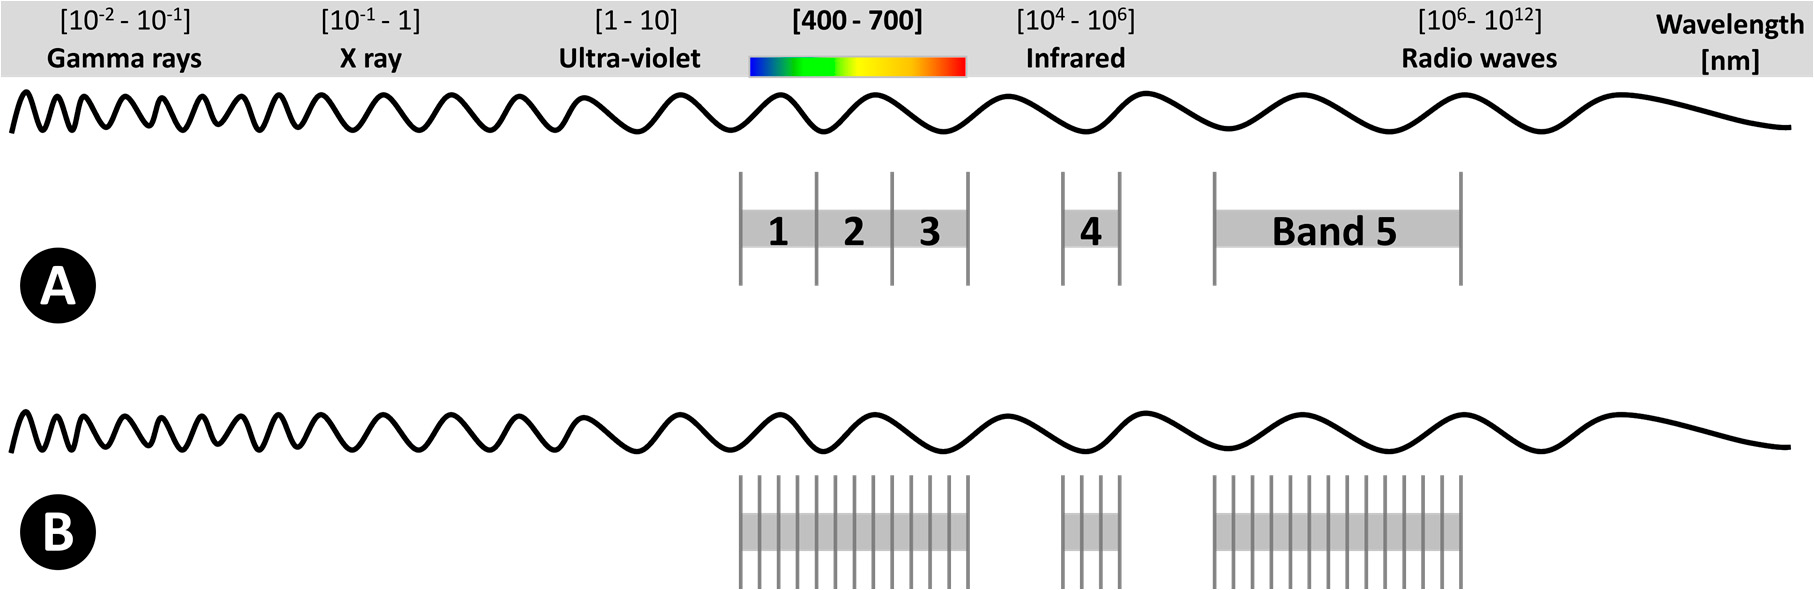
\includegraphics[scale=0.2]{Figs/plan_de_tesis/multivshyper.png}
	\caption{ Representación de los espectros: (A) Multiespectral: 5 
		bandas anchas; y, (B) Hiperespectral: muchas bandas muy estrechas, 
		generalmente entre cientos y miles de ellas. Los dibujos no se 
		encuentran 
		realizados a escala. Imagen tomada de \cite{Adao2017}.}
	\label{fig:spectrus}
\end{figure}


Las cámaras de adquisición de imágenes hiperespectrales estándard utilizan 
redes de difracción o prismas como elementos dispersivos de la luz. La 
distancia requerida entre el sensor de detección y  el componente de difracción 
de la luz, hace que este tipo de cámaras sean muy grandes y muy pesadas, dos 
condiciones que por ejemplo en la industria satelital se quieren optimizar 
fuertemente ya que el costo de la puesta en órbita de los satélites es 
proporcional a su peso y a su tamaño. Estas cámaras suelen ser muy caras y muy 
sensibles a desalinearse debido a las condiciones mecánicas de su construcción. 
Esta última condición se agrava en sistemas de difícil manipulación como lo son 
los satélites, que una vez que se encuentra en órbita, sus componentes ópticos 
ya no puede ser modificados como para corregir una desalineación que empeore la 
calidad de las imágenes capturadas. Además, requieren de una rendija 
para poder obtener una alta resolución espectral, lo que restringe 
significativamente la intensidad de la luz a detectar.

En respuesta a las desventajas de las cámaras estándard de imágenes 
hiperespectrales, aparecieron otro tipo de cámaras que utilizan filtros de 
interferencia de banda y que resultaron en un producto final robusto, compacto, 
de bajo costo y de muy buen rendimiento. Una cámara de vuelo 
de este tipo fue desarrollada en la tesis de licenciatura de Agustina Pose bajo 
la dirección de Hernán Grecco \cite{Pose2017} como se mencionó anteriormente. 
La cámara desarrollada tiene la gran ventaja de no presentar partes móviles, 
evitando posibles desalineaciones de los componentes ópticos. Las partes 
móviles de la cámara que serían útiles para realizar un barrido espectral de 
una cierta escena a capturar, no son necesarias pues el barrido es realiizado 
por el movimiento propio del satélite respecto de la Tierra. El esquema básico 
de este tipo de 
cámaras hiperespectales se muestra 
en la Figura \ref{fig:camsens}. Los filtros de interferencia de banda 
utilizados en este tipo de cámaras deben cumplir ciertos requisitos de calidad 
(no presentar rayones, ni marcas, etc) 
y ciertas características espectrales y de transmisión antes de ser 
incorporados a la carga útil de, por ejemplo, un satélite que va a ser puesto 
en 
órbita. En consecuencia, resulta fundamental caracterizar completamente dichos 
filtros antes de construir las cámaras de la aplicación de interés.

\begin{figure}[H]
	\centering
	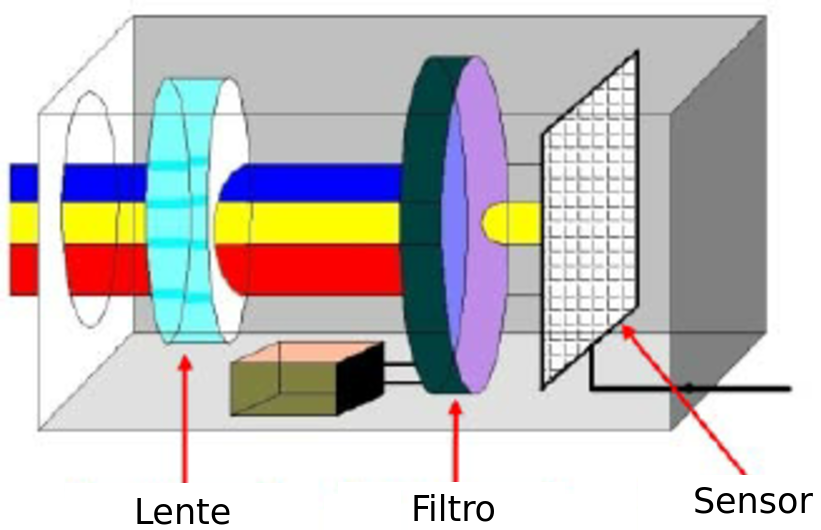
\includegraphics[scale=0.535]{Figs/plan_de_tesis/cam_sens.png}
	\caption{ Esquema de una cámara hiperespectral. El filtro absorbe el 
	espectro completo de la luz incidente salvo la banda espectral que el 
	usuario determina, por lo que sólo las longitudes de onda elegidas 
	atraviesan el filtro y son detectadas por el sensor. \cite{Martinez2008}}
	\label{fig:camsens}
\end{figure}



Debido a las limitaciones de las técnicas de 
medición estándard 
de los espectros de transmisión de los filtros ópticos donde se utilizan 
espectrómetros comerciales, existen tres discrepancias fundamentales 
entre el espectro ''real''\footnote{El espectro ''real'' es 
	el espectro de diseño del filtro para el que fue especialmente construido.} 
	de 
un 
filtro y sus mediciones experimentales realizadas con 
espectrómetros comerciales (Ver Figura \ref{fig:obj1a})\cite{Semrock}. La 
primera discrepancia es el "redondeo" de características espectrales nítidas de 
los filtros. 
Esto se debe al ancho de banda no nulo del haz de la sonda del 
espectrómetro. 


La segunda discrepancia se debe al rango limitado de 
medición de la OD\footnote{La densidad óptica, OD (Optical Density), es un 
	parámetro útil para describir la transmisión de la luz a través de un 
	filtro 
	óptico con una transmisión extremedamente baja. Si T es la transmisión del 
	filtro, que varía entre 0 y 1, se define la densidad óptica como $OD = 
	-$log$_{10} (T)$.} del filtro, que es 
producto de la sensibilidad limitada del espectrómetro. Cuando un filtro 
tiene un valor de OD muy alto, OD $>$ 6, el detector debería medir una 
intensidad de la luz prácticamente nula pero el ruido óptico y electrónico 
propio del detector limita el nivel más bajo de intensidad que puede medir 
con precisión. De esta forma, se puede ver un ruido de piso debido al 
sensor indicando un cierto valor de OD que no coincide con el valor real 
del filtro.

\begin{figure}[H]
	\centering
	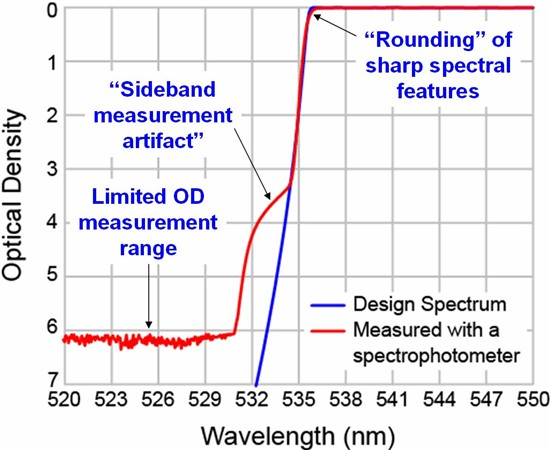
\includegraphics[scale=0.8]{Figs/plan_de_tesis/measurement_of_optical_filter.jpg}
	\caption{Discrepancias entre las mediciones experimentales con 
		espectrómetros 
		comerciales y el espectro ''real'' de un filtro óptico. Adaptado de 
		\cite{Semrock}.}
	\label{fig:obj1a}
\end{figure}

La tercera 
discrepancia es propia de las mediciones de transiciones muy 
pronunciadas. Esto surge 
por el hecho de que el 
haz de la sonda no es monocromático, sino que también tiene bandas 
laterales débiles de longitudes de onda fuera de su ancho de banda 
principal.

Las discrepancias de medición en espectrómetros convencionales 
causan 
importantes problemas al intentar evaluar el rendimiento del filtro para la 
aplicación prevista. 

La elección del instrumento de medición y la técnica 
empleada determinan la precisión de la medición del espectro de transmisión del 
filtro. Al mismo tiempo, determinan la duración y por ende también el costo de 
dichas mediciones, que deben ser compatibles con los tiempos que la industria 
requiere. Esto se puede ver con un ejemplo tomado de \cite{Semrock}. En la 
Figura \ref{fig:may_dists} se muestran cinco mediciones distintas de 
la densidad óptica de un filtro diseñado para bloquear longitudes de onda de 
532 nm con OD $>$ 6 y tener una transición a un estado de alta transmisión 
dentro del $0.5\%$ de la longitud de onda del láser utilizado para excitar la 
muestra, que es de 534.7nm.


\begin{figure}[H]
	\centering
	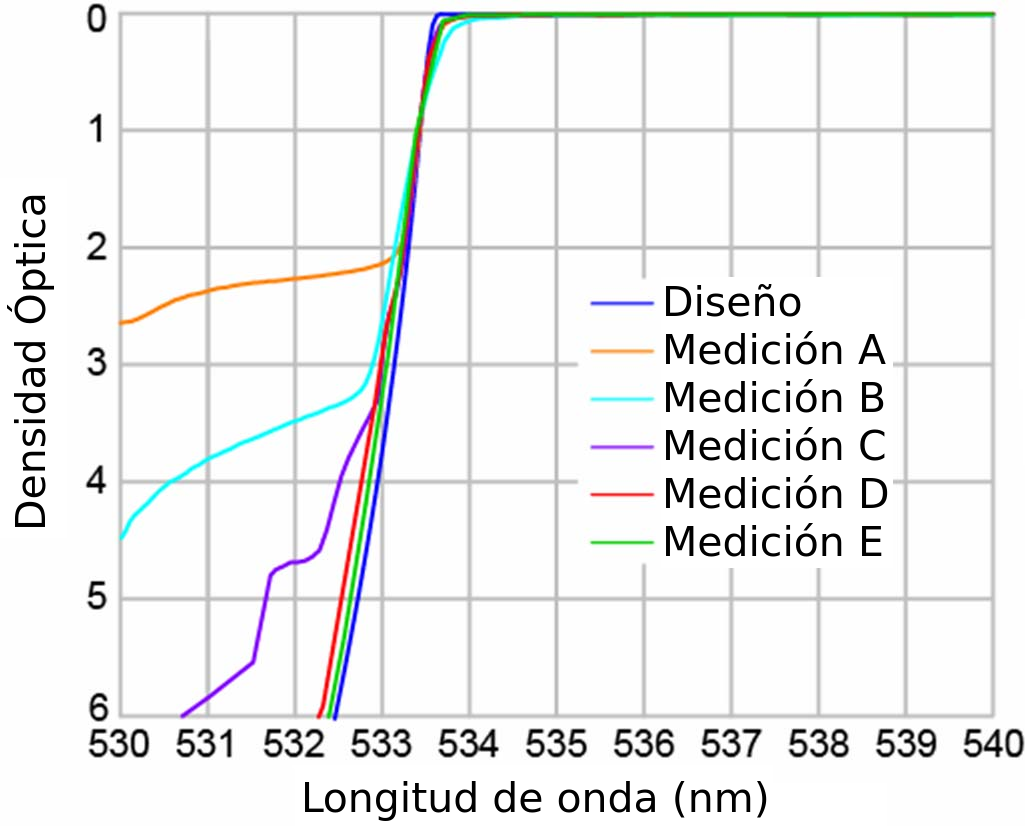
\includegraphics[scale=0.8]{Figs/plan_de_tesis/dists_meds.png}
	\caption{Distintas mediciones de la OD de un filtro LP03-532RE-
		25 RazorEdge de la empresa Semrock. Las mediciones fueron realizadas 
		utilizando tanto espectrómetros comerciales como \textit{custom-made} 
		de la emppresa con una variedad de arreglos experimentales que se 
		explican en el texto. Adaptado de 
		\cite{Semrock}.}
	\label{fig:may_dists}
\end{figure}

Las mediciones del método A fueron realizadas por un espectrómetro de diseño 
propio (\textit{custom-built}) de la empresa,  que tiene un tiempo de 
integración muy corto y una baja resolución, lo que resulta en una 
configuración 
experimental óptima para obtener mediciones de una gran cantidad de filtros de 
prueba. Este método es utilizado para determinar con precisión la longitud de 
onda a partir de la cual el filtro pasa a tener una alta transmisión, es decir, 
localiza la longitud de onda de la transición entre el estado de bloqueo y de 
transmisión del filtro, la longitud de onda de corte. De esta forma, se 
garantiza una cierta uniformidad en un lote de filtros a ser utilizado de una 
forma rápida y eficiente. Ahora bien, como se observa en el gráfico de la 
Figura \ref{fig:may_dists}, el método A posee una sensibilidad muy mala y una 
resolución muy baja, obteniéndose un piso de ruido mayor a OD 2.

El método B utiliza un espectrómetro comercial (Perkin Elmer
Lambda 900) cuyos inconvenientes fueron explicados a partir de las tres 
discrepancias en la Figura \ref{fig:obj1a}. Con este método no se puede 
asegurar que el filtro tenga un 0D $>$ 6 en los 532nm.


Los métodos C y D utilizan el mismo espectrómetro \textit{custom-built}	del 
método A, cuyo principio de funcionamiento básico se muestra en la Figura 
\ref{fig:med_prev}. La diferencia fundamental con el método B que utiliza un 
espectrómetro comercial es que las mediciones con el espectrómetro 
\textit{custom-built} realizan la detección con una cámara CMOS de bajo ruido, 
que consiste en un arreglo de detectores, por lo que puede medir en un rango 
muy grande de longitudes de onda simultáneamente. Este método permite en 
consecuencia obtener mediciones en un rango espectral muy grande, con una 
cierta resolución en un cierto tiempo de integración, de forma muy rápida.
El inconveniente fundamental de este método es que al utilizar una fuente de 
iluminación de banda ancha, si el filtro de prueba tuviera, por ejemplo, una 
autofluorescencia apreciable \cite{Shah2017}, podría interferir con una 
medición precisa de la transmisión de la muestra.


\begin{figure}[H]
	\centering
	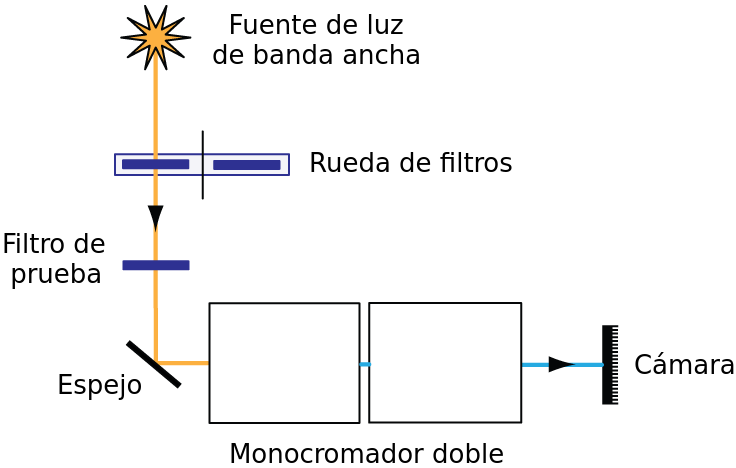
\includegraphics[scale=0.8]{Figs/plan_de_tesis/med_mets_prevs.png}
	\caption{Diseño básico de un espectrómetro \textit{custom-built} que 
	utiliza una fuente de iluminación de banda ancha y permite la recolección 
	de una 		amplia gama de
		longitudes de onda simultáneamente con un conjunto de detectores 
		situados en la cámara. Este 
		arreglo experimental permite una medición más rápida con un piso de 
		ruido y una resolución fijas. Adaptado de 
		\cite{Semrock}.}
	\label{fig:med_prev}
\end{figure}




Ahora bien, dependiendo de la aplicación, las limitaciones en las mediciones 
del espectro de transmisión de los filtros pueden ser determinantes o no. En el 
presente proyecto se quiere determinar el arreglo experimental óptimo pero que 
sea compatible con los tiempos y costos de producción de la industria satelital.

En ciertos filtros y aplicaciones, resulta de vital importancia 
el 
nivel de bloqueo de ciertos rangos de longitudes de onda pero no así la 
suavidad de la transición entre el bloqueo y la transmisión. Por ejemplo, en 
sistemas de 
imágenes de fluorescencia los espectros de absorción y emisión del fluróforo 
podrían estar lo suficientemente alejados como para que resulte fundamental que 
los filtros de banda de la señal de respuesta (de emisión) de la muestra tengan 
un bloqueo muy alto en la banda de la señal de excitación y así lograr una 
relación entre la señal y el ruido de adecuada proporción \cite{Grecco2016}. 

Los filtros 
diseñados para estas aplicaciones podrían tener decenas de OD de bloqueo pero 
en 
la práctica incluso el más pequeño de los defectos físicos en los 
recubrimientos ópticos (\textit{coatings}) o en el montaje, así como el bajo 
nivel de control de luz parásita a nivel del sistema, puede limitar el 
bloqueo alcanzable a valores mucho menores que los del diseño original, en el 
rango de aproximadamente OD 6 a quizás 10.%(forma indirecta de medir los scrath 
%and dig!!**))) 

Dado que los espectrómetros 
comerciales estándard tienen una medición de OD de rango limitado debido al 
ruido de fondo del instrumento, se propone un arreglo experimental inicial para 
poder medir los niveles de bloqueo más altos con precisión como se muestra en 
la Figura \ref{fig:su} y que resulta compatible con la producción industrial 
deseada por su simplicidad.


\begin{figure}[h!]
	\centering
	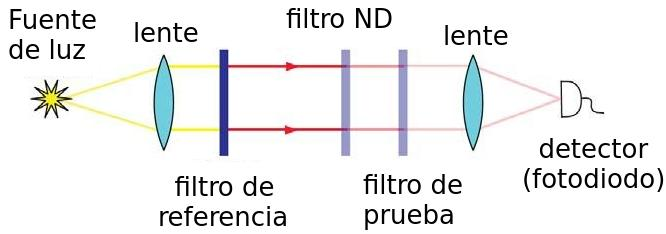
\includegraphics[scale=1.0]{Figs/plan_de_tesis/setup_u.jpeg}
	\caption{Arreglo experimental compatible con la producción industrial para 
	medir valores de 
	OD altos.}
	\label{fig:su}
\end{figure}

El método experimental de la Figura \ref{fig:su} se denomina 
\textit{complementary filter method}. Un haz de 
luz de banda ancha, de una lámpara QTH 
(\textit{Quartz-Tungsten Halogen}) ó de arco, aproximadamente colimado por una 
lente  es filtrado utilizando un filtro 
de referencia ampliamente bloqueador, que es esencialmente un filtro de banda 
con su banda de paso superpuesta a la región del espectro del filtro de prueba 
que se quiere analizar donde la medición de valores de OD altos son necesarios. 
La luz transmitida es enfocada con una lente convergente en un detector de bajo 
ruido capaz de medir niveles de intensidad de luz muy pequeños, como un 
fotodiodo de gran área con un circuito amplificador de bajo ruido ó un tubo 
fotomultiplicador (PMT).


Las mediciones se realizan de la siguiente manera. En primer lugar, se mide la 
intensidad de la señal en el detector con solo el filtro de referencia y un 
filtro calibrado de densidad neutra (ND) en la trayectoria de la luz. El filtro 
ND sirve para reducir el nivel de la intensidad de la luz en el detector en 
una cantidad calibrada de forma tal que el bias \footnote{El bias del 
detector es el valor medido por el instrumento cuando no hay ninguna fuente 
de luz incidiendo sobre él, es el valor de \textit{offset} que se le suma a 
cualquier 
medición.} del rango 
dinámico limitado alcanzable por el detector sea reducido para alcanzar los 
niveles de la señal que el detector va a ver cuando se coloquen los filtros de 
prueba. En particular, con un filtro ND 3, el rango dinámico del detector tiene 
que ser de $10^{6}$ para medir hasta un valor de OD 9 de bloqueo. En segundo 
lugar, se retira el filtro ND y se lo reemplaza por el filtro de prueba para 
realizar una nueva medición de la intensidad con el detector. El cociente entre 
las dos mediciones de intensidad de la luz es igual al valor de OD del filtro 
de prueba, en el rango espectral del filtro de referencia.


\section*{Actividades y Metodología}

\hspace{0.5cm}En el presente trabajo de tesis se desarrollarán múltiples 
arreglos 
experimentales para caracterizar el espectro de transmisión de distintos 
filtros de prueba que dispone el LEC, utilizando técnicas de medición en línea 
con los papers y patentes de la actualidad. Se automatizará la adquisición de 
las mediciones y se incorporará al arreglo experimental inicial un sistema de 
detección de defectos de los filtros, utilizando una cámara de bajo costo del 
laboratorio para realizar las primeras pruebas. 

Una vez caracterizado tanto el espectro como los defectos de los filtros, se 
diseñará y construirá un primer prototipo de un sistema integral de 
caracterización para ser aplicado con los filtros que utiliza la empresa 
Satellogic en sus cámaras hiperespectrales. Se estudiará la aplicabilidad de 
este prototipo en distintos casos.

Utilizando el prototipo del sistema integral de caracterización de los filtros 
se desarrollará un método y criterios para decidir si un filtro puede ser 
incorporado a la cámara utilizada en los satélites.

Como aplicación de este proyecto de tesis se utilizarán las cámaras 
hiperespectrales de la empresa Satellogic, cuyos filtros van a ser 
caracterizados con el sistema integral que se va a desarrollar, y se tomarán 
imágenes en tierra utilizando algoritmos de HDR y de búsqueda de 
características.  Y, finalmente se realizará una caracterización de los filtros 
en su posición final en las cámaras de vuelo del satélite.

El cronograma mensual de trabajo se muestra en la siguiente Tabla:

%\begin{tcolorbox}[tab2,tabularx={X||Y|Y|Y|Y|Y|Y|Y|Y|Y|Y|Y|Y},title= 
%\textbf{Cronograma mensual de actividades propuestas},boxrule=0.5pt]
%	\textbf{Actividad} & \textbf{4} & \textbf{5} & \textbf{6} & 
%	\textbf{7} & \textbf{8} & \textbf{9} & \textbf{10} & \textbf{11} & 
%	\textbf{12}      
%	\\\tcbline\tcbline
%	Revisión del estado del arte   &  \checkmark    &  & & & & & & & \\\tcbline
%	Caracterización de los espectros de transmisión de los filtros    &   & 
%	\checkmark & \checkmark
%	& \checkmark & & & & &\\ \tcbline
%	Determinación de defectos de los filtros (\textit{scratch and dig})     &   
%	&  & \checkmark & \checkmark & & & & &\\ \tcbline
%	Diseño y construcción del primer prototipo del sistema integral de 
%	caracterización de los filtros    &   
%	&  &  & \checkmark & \checkmark & & & &\\ \tcbline
%	Implementación del sistema integral en las cámaras de Satellogic. 
%	    &   
%	&  &  &  & \checkmark & \checkmark & \checkmark & &\\\tcbline
%	Procesamiento de imágenes haciendo HDR y búsqueda de características  &   
%	&  &  &  & \checkmark & \checkmark & \checkmark & \checkmark &\\\tcbline
%	Caracterización de los filtros en su posición final en las cámaras de vuelo 
%	del satélite   &   
%	&  &  &  & &  &  & \checkmark & \checkmark \\\tcbline
%\end{tcolorbox}



\section*{Factibilidad}

\hspace{0.5cm}El lugar de trabajo donde el tesista va a desarrollar sus 
actividades es el 
Laboratorio de Electrónica Cuántica (LEC) del Departamento de Física de la 
Facultad de Ciencias Exactas y Naturales, UBA. El LEC cuenta con diversos 
equipos de uso general en óptica y electrónica y algunos de uso específico para 
aplicaciones en investigación de física básica. Entre los equipos de uso 
relevante para el presente proyecto se pueden encontrar mesas ópticas de 
suspensión neumática, un microscopio invertido automático Zeiss Observer Z1, 
diversas placas de adquisición y procesamiento (NI y Red Pitaya, Raspberry Pi y 
Arduino), cámaras científicas y de bajo ruido (Apogee U2000, QHY183M), 
elementos de óptica para la construcción de instrumentos (lentes, filtros, 
objetivos de microscopio, optomecánica, láseres y leds). Adicionalmente, el 
laboratorio cuenta con acceso a un microscopio confocal de la firma Olympus, 
modelo FV1000 equipado con una platina motorizada, cámara ambiental y cámara 
CCD.
 
El director de la presente tesis es director del LEC y es experto en temas de 
óptica y fotofísica, áreas principales del proyecto. Además, tiene la 
experiencia de haber dirigido a una estudiante que realizó la tesis en conjunto 
con el LEC y la empresa Satellogic, resultando en una experiencia exitosa.

El tesista se encuentra cursando actualmente sus últimas dos materias de la 
carrera: 
Estructura de la Materia 4 e Instrumentación y Control.


\renewcommand\bibname{Referencias Bibliográficas}
\bibliographystyle{apalike}
\bibliography{refs}


\chapter{Primer prototipo del equipo y caracterización de los espectros de transmisión}

\chapter{Spectral GUI y software del primer prototipo: Integración clases del espectrómetro y de los motores de thorlabs - Implementación con Multithreading}

\chapter{Desarrollo XZStage y calibración - Desarrollo del software integrando el arduino con algoritmos asincrónicos}

\chapter{Montaje Microespectrómetro, caracterización resolución espacial y calibración}

\chapter{Integración cámara al microespectrómetro}

\chapter{Cuantificación de los defectos a partir de las imágenes tomadas con el ZEISS con scikit-image y OpenCV}

De forma complementaria a las mediciones del microespectrómetro, se tomaron imágenes por transmisión del filtro con un microscopio ZEISS Axio Observer Z1 como se muestra en la Figura \ref{fig:ZEISSdellabo}, utilizando el objetivo ZEISS de magnificación 10X. 

De acuerdo a la calibración de fábrica del ZEISS, 1 pixel de la imagen equivale a 0.586 micrones. 
\vspace{1cm}
\todo[inline]{CALIBRAR ZEISS con alguna reglita de calibración}
\vspace{1cm}





\begin{figure}[H]
	\centering
	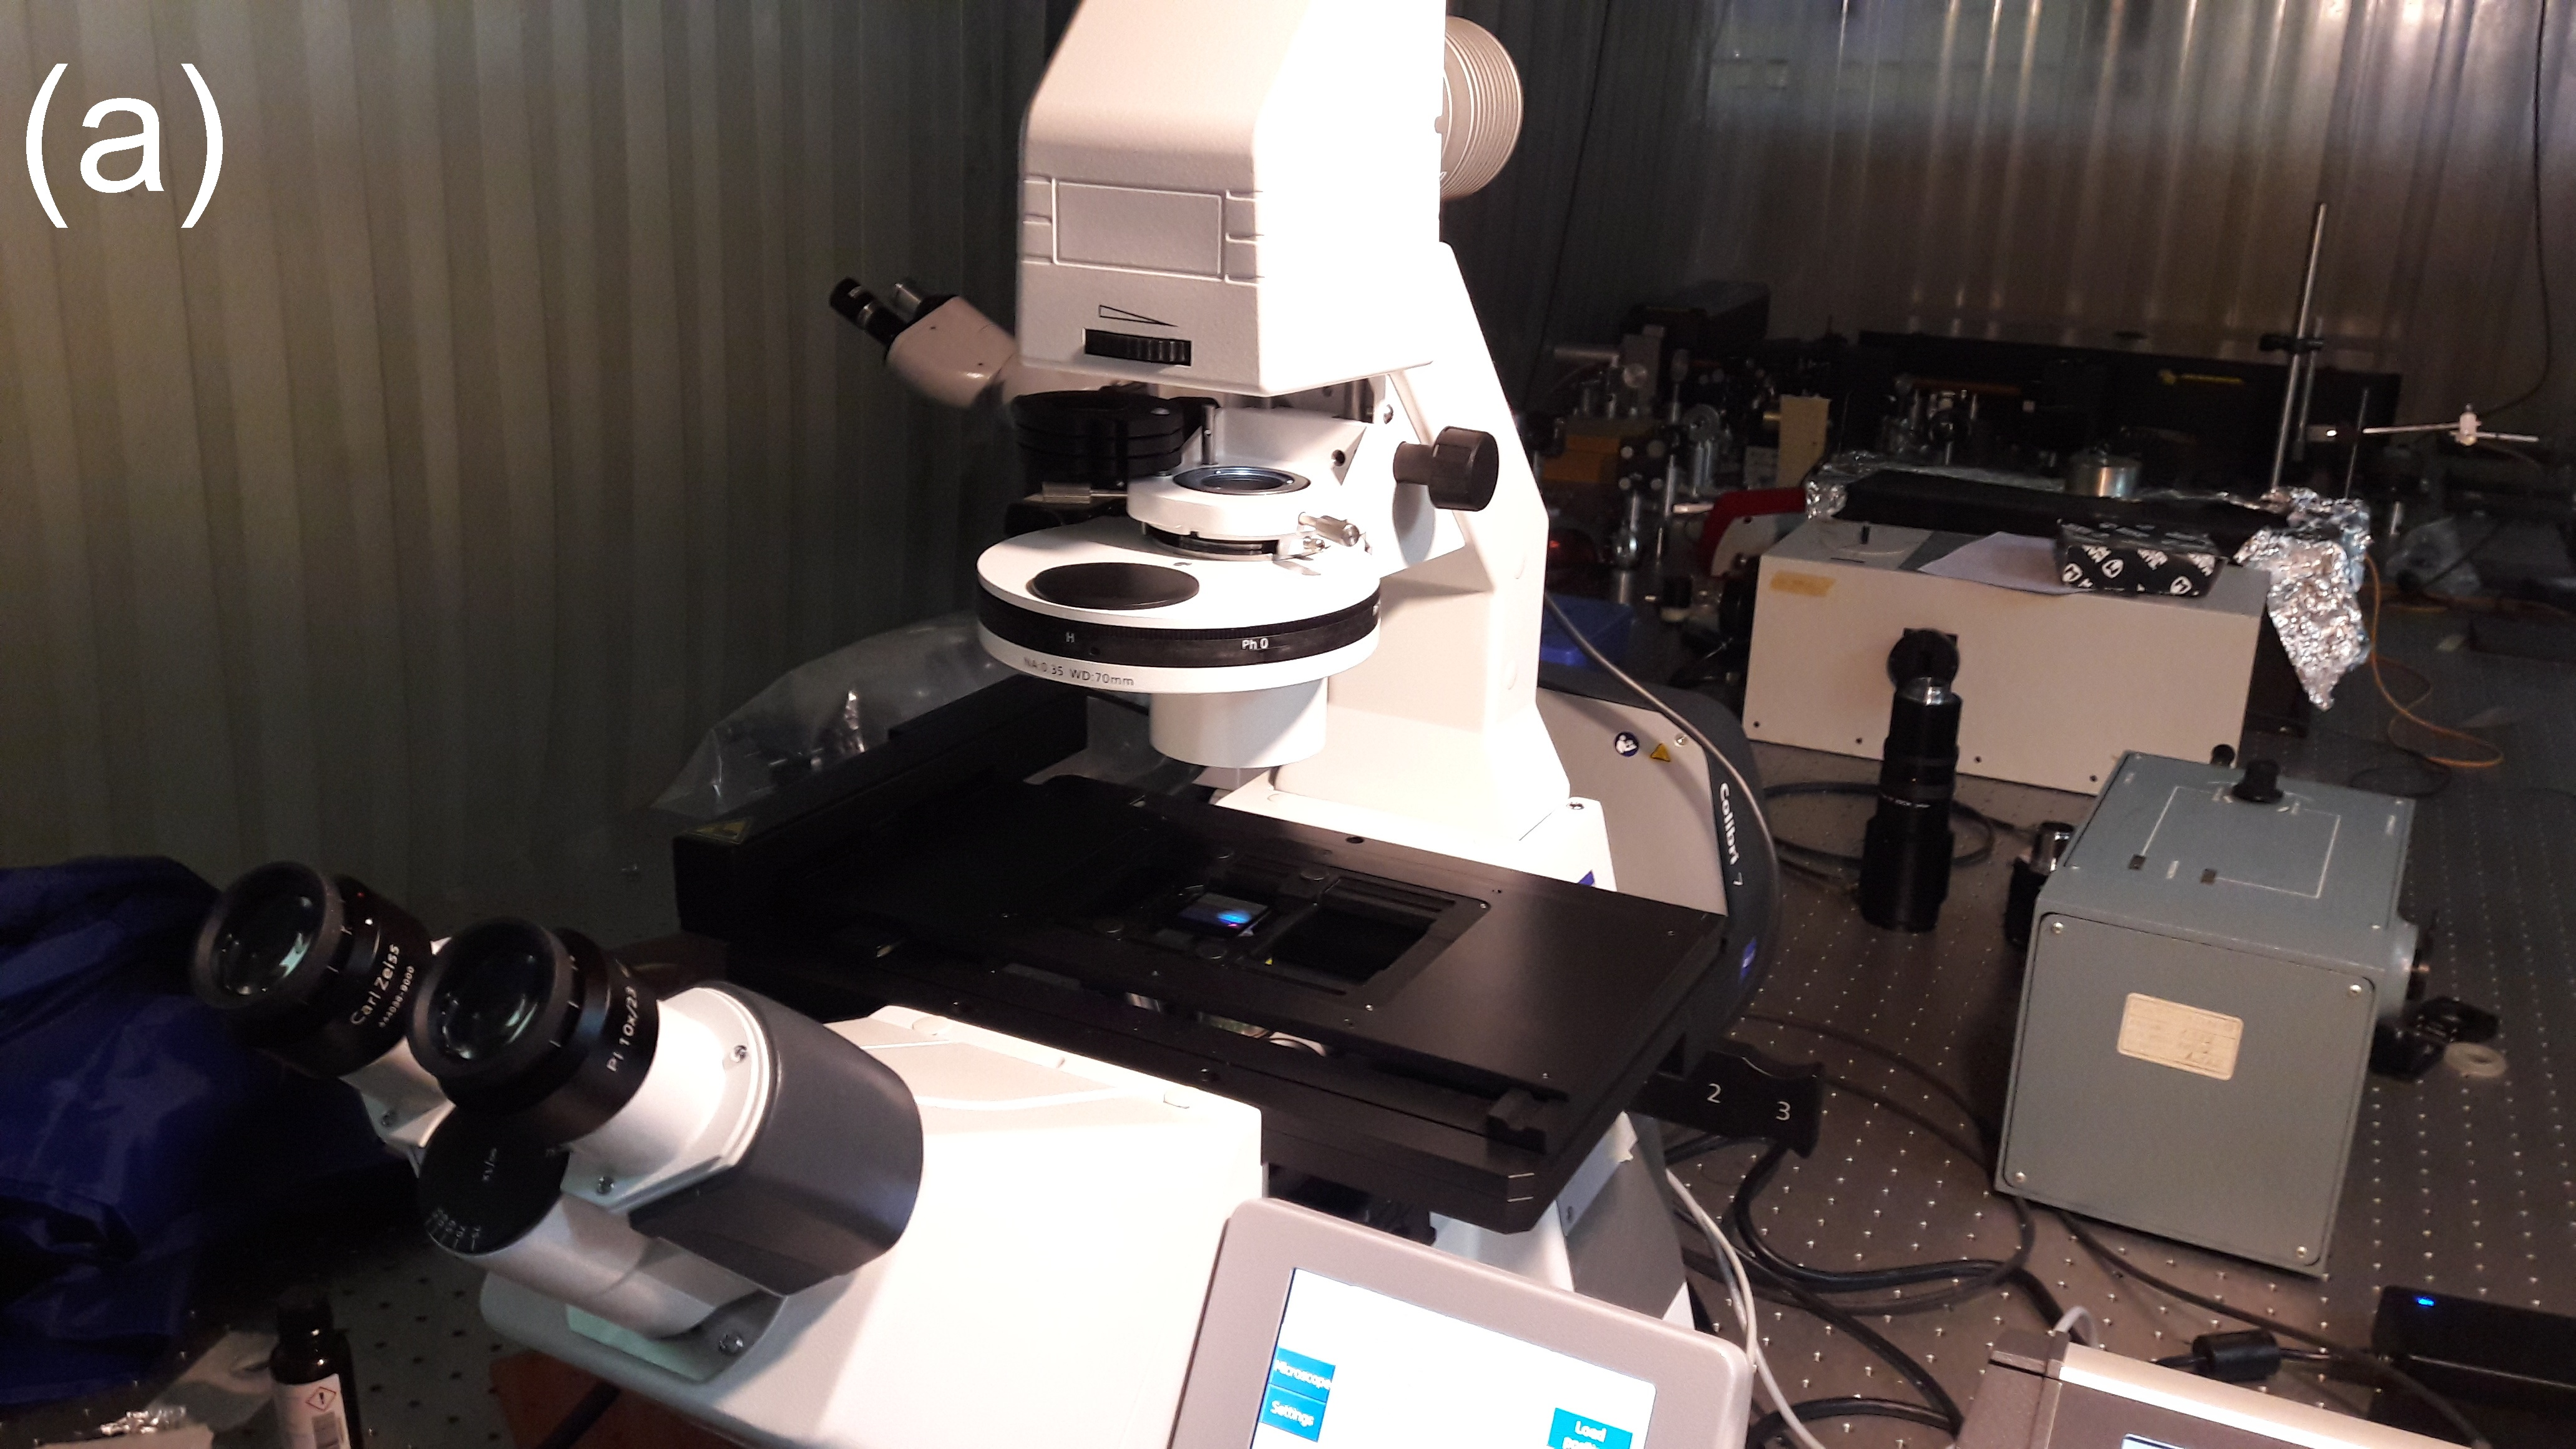
\includegraphics[scale=0.1]{Figs/defectosZEISS/b.jpg}
	\caption{ }
	\label{fig:ZEISSdellabo}
\end{figure}

Se montó el filtro sobre el portamuestras del microscopio como se muestra en la Figura \ref{fig:filtroenZEISS}.
Utilizando el software ZEN PRO 2.5.

\vspace{1cm}
\todo[inline]{chequear versión del ZEN PRO y tomar screenshot del gráfico del histograma - rango dinámico}
\vspace{1cm} 

Luego de poner en foco una de las superficies del filtro con el software y refinando la distancia entre el objetivo y el filtro con las perillas manuales del microscopio, se realizaron distintos 'barridos' del filtro.

\begin{figure}[H]
	\centering
	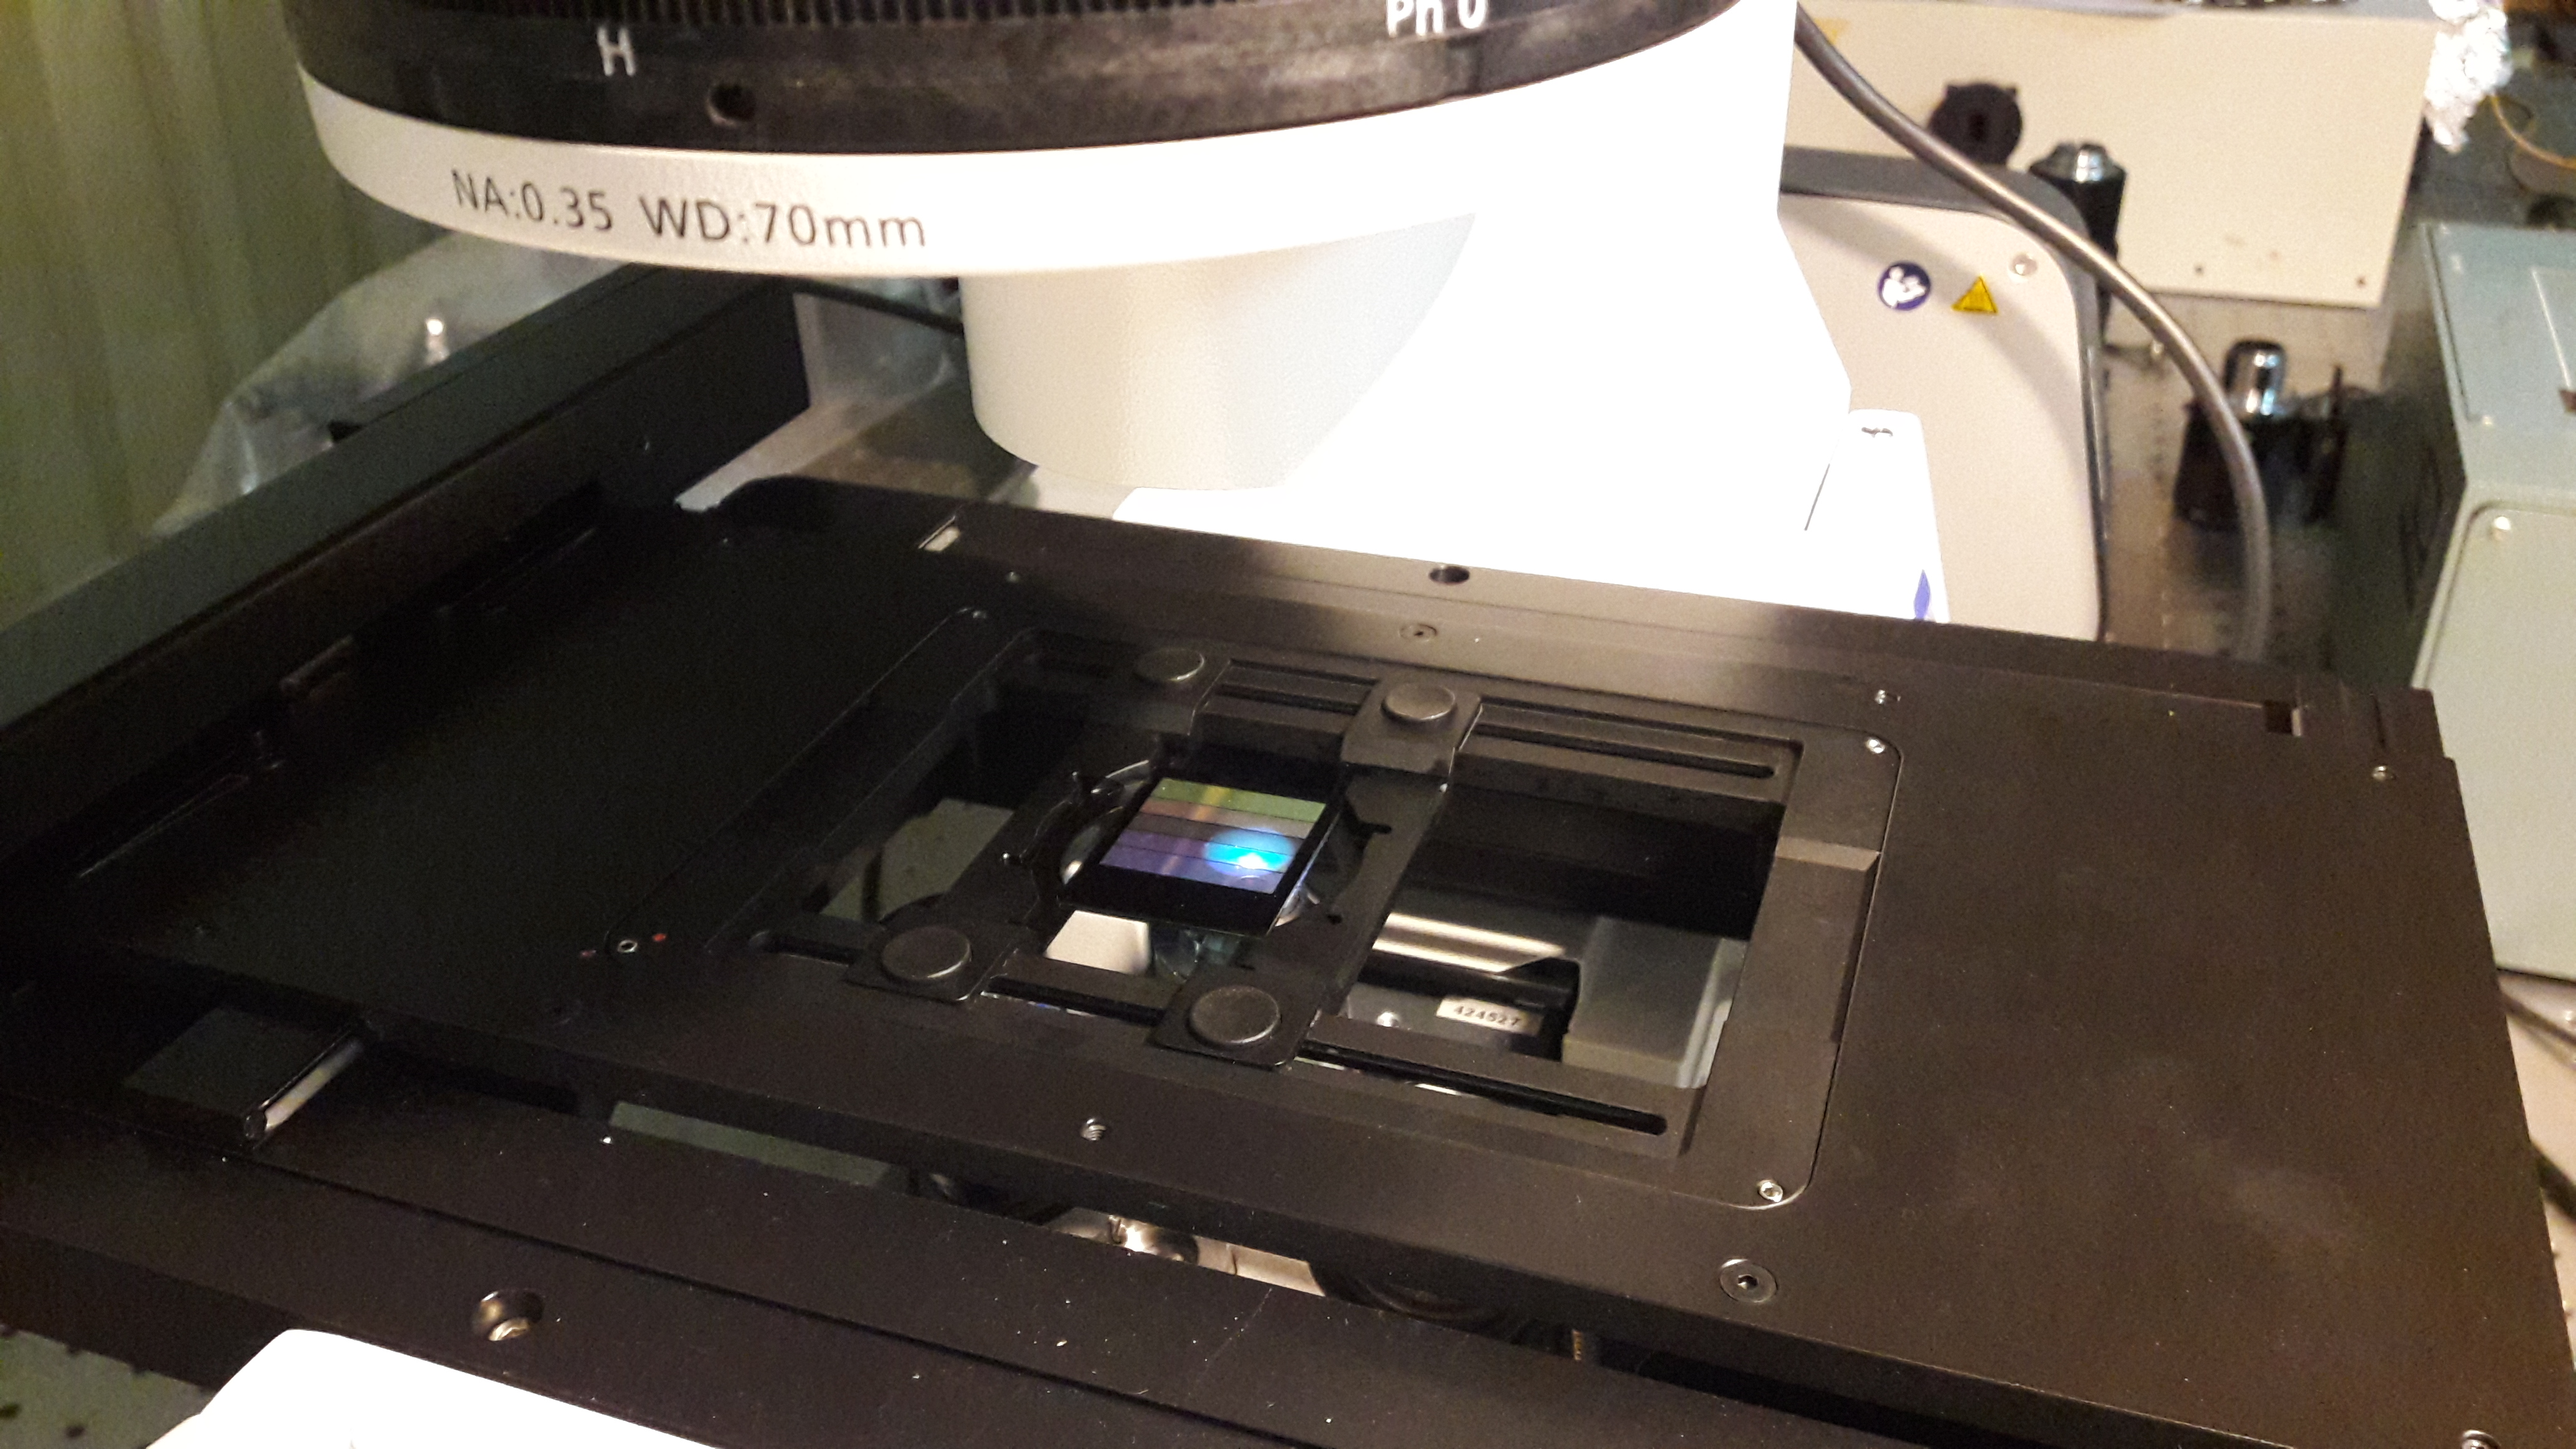
\includegraphics[scale=0.1]{Figs/defectosZEISS/a.jpg}
	\caption{ }
	\label{fig:filtroenZEISS}
\end{figure}

\chapter{Conclusiones}

\chapter{Trabajo a futuro}



\end{document}

